\chapter{Cloud Computing} 
\label{ch:cloud}
Das letzte Kapitel hat deutlich gemacht, welche Anforderungen im Hochschulsport an ein Software System gestellt werden, sowie welchen Dynamiken und Besonderheiten das fachliche Umfeld unterliegt. In diesem Kapitel soll ein Verständnis für unterschiedliche Softwarearchitektur und Vertriebsmodelle geschaffen werden. Dabei soll vor allem auf das Thema Cloud Computing eingegangen werden, welches an Bedeutung gewinnt und Gegenstand vieler akademischen und wirtschaftlichen Beiträgen in der Fachpresse ist. 
\\

Für den Begriff Cloud Computing finden sich in der Literatur vielfältige Definitionen. [Beispiel] Die häufigste Verwendung findet jedoch die Definition des National Institute of Standards and Technology in der Form:

\begin{quote}
	Cloud computing is a model for enabling ubiquitous, convenient, on-demand network access to a shared pool of configurable computing resources (e.g., networks, servers, storage, applications, and services) that can be rapidly provisioned and released with minimal management effort or service provider interaction. This cloud model is composed of five essential characteristics, three service models, and four deployment models.
\end{quote} \cite*[vgl.][S.2]{Mell.2011}\\


Bevor die Merkmale, Service  und Bereitstellungsmodelle im Detail erläutert werden, ist es jedoch wichtig zu verstehen, woher die Notwendigkeit bestand ein neues Modell zu erschaffen.

\section{Herausforderungen traditioneller Architekturen}


\section{Merkmale}
On-demand self-service\\
Broad network access\\
Resoruce pooling\\
Rapid elasticity\\
Measured service
\cite*[vgl.][S.2]{Mell.2011}

\section{Service Modell}
In der Definition von \cite*[S.2]{Mell.2011} sind drei unterschiedliche Service Modelle beschreiben, die sich in der Cloud Community etabliert haben. Diese decken sich mit den Kategorisierungen von \cite[S. 28]{Tharam.2010} und \cite[S. 878]{Jadeja.2012}.

	\begin{figure}[h]
		\centering
		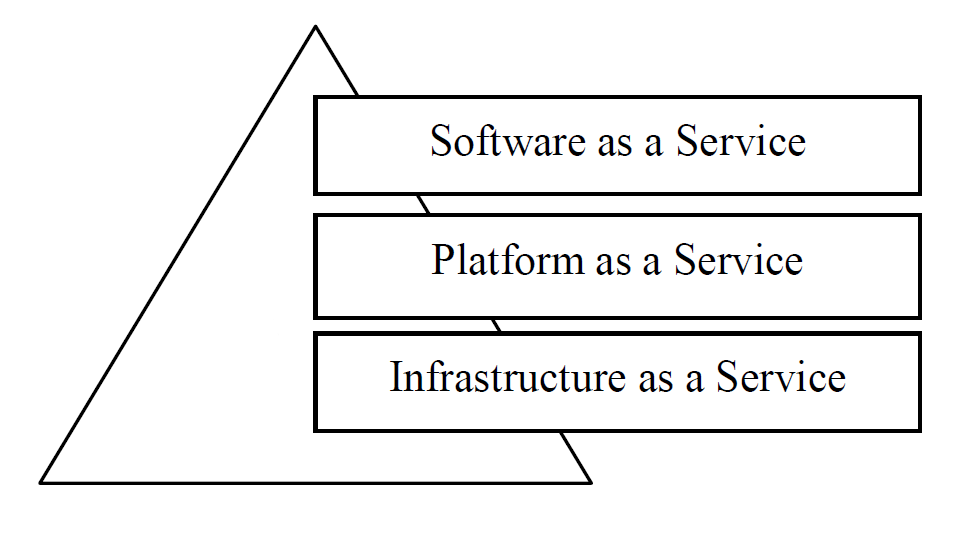
\includegraphics[width=0.7\linewidth]{images/cloud_computing_pyramide}
		\caption{3-Ebenen Modell von Cloud Computing}
		\label{fig:CloudComputingPyramide}
	\end{figure}


\textbf{Software as a Service (SaaS)} stellt eine Anwendung in der Cloud bereit, die von Nutzern verwendet werden kann, ohne eine eigene Installation vornehmen zu müssen. Der Nutzer hat dabei keinen Zugriff auf die Cloud Infrastruktur. Wichtige Merkmale einer SaaS Anwendungen sind Netzwerk basierter Zugriff, Nutzer können limitierte spezifische Konfigurationen vornehmen und sind meistens als Multi-Tenancy-System aufgebaut. Beispiele sind Anwendungen wie SalesForce.com, Google Mail, Google Docs, Office 365, Quicken Online, etc.
\\

\textbf{Platform as a Service (PaaS)} bezeichnet Software und Entwicklungs Tools die der Nutzer verwenden kann, um eigene Anwendungen zu entwickeln und zu veröffentlichen. Der Nutzer hat dabei keinen Zugriff auf die darunter liegende Cloud Infrastruktur, kann jedoch im Vergleich zu SaaS die eigene Anwendung frei konfigurieren. Beispiele für PaaS Services ist Google AppEngine.
\\

\textbf{Infrastructure as a Service (IaaS)} ist die unterste Ebene der Cloud Computing Pyramide. Dem Nutzer wird virtualisiert Hardware wie Datenspeicher, Virtuelle Maschinen, Netzwerke, etc. zur Verfügung gestellt, die frei verwendet werden können. IaaS Services werden gewöhnlich auf pay-per-use Basis bezahlt. Amazon EC2, VMWare und Windows Azure sind nur einige Beispiele.
\\

In einigen Fällen werden diese drei Ebenen noch um zusätzliche Service Formen ergänzt. So verwendet \cite[S. 28]{Tharam.2010} noch die Einteilung in storage as a Service (DaaS) während \cite[S. 123]{Mahmood.2011} von "other Provision as Service" spricht und darunter Formen wie Storage as a Service, Database as a Service, Security as a Service, Communication as a Service, etc gruppiert. All diese Services können jedoch auch spezialisierte IaaS Services angesehen werden.


\section{Bereitstellung Modell}
Ein weiterer wichtiger Punkt in der Definition von Cloud Computing ist das Bereitstellungsmodell, das primär die Art beschreibt, wer Zugriff hat.

	\begin{figure}[h]
		\centering
		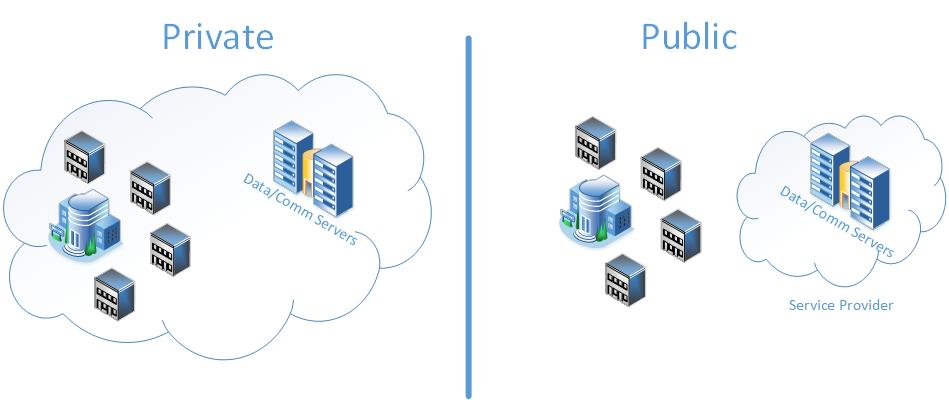
\includegraphics[width=0.9\linewidth]{images/private_public_cloud}
		\caption{Public und Private Cloud Architektur}
		\label{fig:PublicPrivateCloud}
	\end{figure}

\subsection{Private Cloud}
Als Private Cloud wird das Szenario beschrieben, wenn die Infrastruktur nur von einem Kunden genutzt wird. Im Normalfall ist sie im Organisationseigenen Rechenzentrum beheimatet. Sicherheit, Datenschutz, Wartung sind so einfacher durch eigenes Personal oder externe Dienstleister zu organisieren. Die Private Cloud lässt sich daher mit einem Intranet vergleichen. \cite[S. 879]{Jadeja.2012} \\
\cite{Tharam.2010} nennen fünf Gründe, die für eine Private Cloud sprechen können:
\begin{enumerate}
\item Maximieren und optimieren bestehender, eigenen Ressourcen
\item Sicherheitsbedenken und Datenschutz
\item Datentransferraten
\item Vollständige Kontrolle über kritische Aktivitäten
\item Forschungs- und Ausbildungszwecke
\end{enumerate}

\subsection{Public Cloud}
Dieses Modell ist derzeit am häufigsten verbreitet. Nutzer können die Cloud über ein Interface ansteuern und bezahlen für die Dauer der genutzten Services. Im Vergleich zu anderen Modellen ist die Public Cloud weniger sicher, da sie offen für bösartige Angriffe ist. Bekannte Public Cloud Anbieter sind Amazon EC2, S3, Google AppEngine, Force.com und Microsoft Azure. \\
(vgl. \cite{Jadeja.2012} und \cite{Tharam.2010})
	
\subsection{Hybrid Cloud}
Bei der Hybrid Cloud handelt es sich aus einer Kombination aus zwei oder mehr Cloud Arten, die für sich selbst existieren, aber miteinander verbunden sind. Dadurch lassen sich einfach eine Private und Public Cloud kombinieren, sodass Sicherheitsanforderungen gerecht geworden werden kann ein "outsourcing" weniger kritischer Teile in eine Public Cloud jedoch nichts im Wege steht.\\
Hybrid Clouds sind die Treiber zur Notwendigkeit einer Standardisierung und Cloud Interoperabilität.

	\begin{figure}[h]
		\centering
		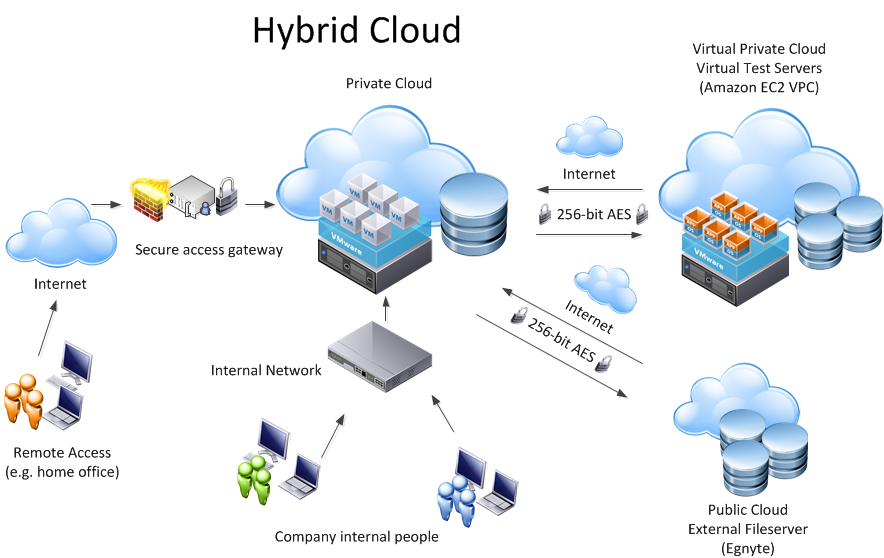
\includegraphics[width=0.9\linewidth]{images/hybrid-cloud-architektur}
		\caption{Hybrid Cloud Architektur}
		\label{fig:HybridCloud}
	\end{figure}


Community Cloud\\

\section{Vorteile}
\section{Probleme und Herausforderungen}
\subsubsection{Sicherheit und Datenschutz}

\section{SaaS Anwendungen}
\subsection{Monolitische versus service basierte Architekturen}
\subsection{Herausforderungen}
\subsubsection{Availability}
\subsubsection{Data management}
\subsubsection{Design and Implementation}
\subsubsection{Messaging}
\subsubsection{Management and Monitoring}
\subsubsection{Performance and Scalability}
\subsubsection{Resiliency}
\subsubsection{Security}


